\mysubsection{Trajectoires}

Dans le cadre d'une t\^{a}che robotique, le mouvement de l'outil dans l'espace est d\'{e}fini par une s\'{e}quence de points travers\'{e}s dans temps. Cette s\'{e}quence et son historique temporel est d\'{e}sign\'{e} par \textbf{trajectoire}. Une t\^{a}che est g\'{e}n\'{e}ralement d\'{e}finie comme le mouvement entre une s\'{e}rie de points vis\'{e}s, par exemple « Aller de la position initiale au point A, s'approcher de la pi\`{e}ce jusqu'au point B, fermer l'outil en saisissant la pi\`{e}ce, aller au point C en portant la pi\`{e}ce~», et l'objectif de la g\'{e}n\'{e}ration de trajectoire est de calculer le chemin travers\'{e} dans le temps parmi des points interm\'{e}diaires et ses respectifs temps. Une fois calcul\'{e}e, la trajectoire est mise comme r\'{e}f\'{e}rence \`{a} l'entr\'{e}e de la commande afin que l'effecteur suive le chemin souhait\'{e}.

La figure \ref{eller1} montre le sch\'{e}ma-bloc usuel pour un g\'{e}n\'{e}rateur de Trajectoire dans l'espace op\'{e}rationnel avec une commande articulaire, o\`{u} $\bm{q}(t)$ est le vecteur de positions articulaires et $\bm{p}(t)\ $est le vecteur des positions cart\'{e}siennes de l'outil. Le sch\'{e}ma est assez simplifi\'{e}, il n'inclue pas le vecteur d'orientation, mais la commande d'orientation est faite d'une fa\c{c}on assez pareille.
\\

\begin{figure}[H]	%Botar a figura aqui
	\captionsetup{justification=centering,margin=1cm}
	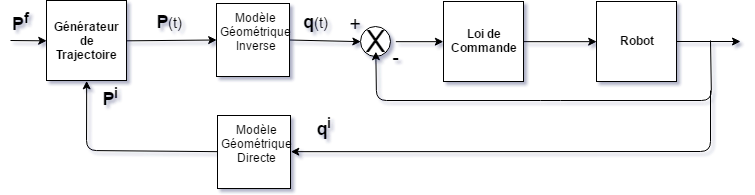
\includegraphics[width=\textwidth]{TrajFig1.png}
	\caption{Sch\'{e}ma-bloc du syt\`{e}me avec le g\'{e}n\'{e}rateur de trajectoires}
	\label{eller1}
\end{figure}


La trajectoire peut \^{e}tre d\'{e}finie en termes de coordonn\'{e}s articulaires ou cart\'{e}siennes, o\`{u} la premi\`{e}re est mieux adapt\'{e} pour un chemin libre entre deux points et la deuxi\`{e}me pour un chemin contraint. Dans ce travail on a d\'{e}cid\'{e} de g\'{e}n\'{e}rer les trajectoires en coordonn\'{e}es cart\'{e}siennes, ce qui demande une commande en espace op\'{e}rationnel ou l'utilisation du mod\`{e}le g\'{e}om\'{e}trique inverse, pour les convertir en coordonn\'{e}es articulaires. 

A part les contraintes g\'{e}om\'{e}triques de la trajectoire, il y a les contraintes temporelles, c'est-\`{a}-dire, contraintes par rapport aux vitesses et acc\'{e}l\'{e}rations en chaque point de la trajectoires et dur\'{e}es maximales du mouvement. Un des principes de conception d'un g\'{e}n\'{e}rateur de trajectoire c'est l'utilisation de trajectoires lisses, une fois que physiquement c'est impossible de traverser l'espace de fa\c{c}on non-continue. En plus on utilise souvent courbes continues en vitesse et acc\'{e}l\'{e}ration afin de minimiser les soucis par rapport aux vibrations et r\'{e}sonances m\'{e}caniques. Afin d'am\'{e}liorer les vitesses, plusieurs g\'{e}n\'{e}rateurs de trajectoire utilisent techniques d'interpolation polynomiale et spline, mais dans le cadre de ce travail on ne les utilisera pas.

\mysubsubsection{Choix de conception et Mise en {\OE}uvre}

Inspir\'{e} par les choix de conception des robots Fanuc, on a d\'{e}cid\'{e} de mettre en {\oe}uvre un g\'{e}n\'{e}rateur de trajectoires avec trois fonctions basiques~: trajectoire lin\'{e}aire entre 2 points, trajectoire circulaire entre 2 points avec un point interm\'{e}diaire et trajectoire en arc de cercle entre 2 points avec un point interm\'{e}diaire. Avec ces trois types de trajectoire le robot sera capable de r\'{e}aliser toutes ses t\^{a}ches.

\mysubsubsection{Trajectoire Lin\'{e}aire}

Le type plus simple de trajectoire, la trajectoire lin\'{e}aire consiste en aller d'un point initial ${\bm{P}}^{\bm{i}}$${}^{ }$au point final ${\bm{P}}^{\bm{f}}$ en suivant une ligne droite, o\`{u} tous les deux points sont vecteurs tridimensionnels et appartiennent \`{a} l'espace op\'{e}rationnel du robot. Soit $\bm{t_f}$ le temps total du mouvement, la trajectoire peut \^{e}tre d\'{e}crite analytiquement par:
\[\bm{p}(t)=({\bm{p}}^f{-\bm{p}}^i) r(t)+\ {\bm{p}}^i\ \ \ ,\ \ \ 0\ge t\ge t_f\] 
\pagebreak\\
O\`{u} r(t) est une fonction monotone continue du temps avec les conditions limites suivantes:
$$ r(0)=0 $$
$$ r(t_f)=1 $$

On peut facilement observer que $\bm{p}(0)=\ {\bm{p}}^{\bm{i}}\ $et que$\ \bm{p}(t_f)=\ {\bm{p}}^{\bm{f}}$, alors la contrainte g\'{e}om\'{e}trique est satisfaite. Pour satisfaire les contraintes de temps on d\'{e}finira $r(t)$ comme un polyn\^{o}me d'interpolation de ${5}^{\grave{e}me}$ d\'{e}gr\'{e}e avec les caract\'{e}ristiques suivantes~:
\[\dot{r}(0)= 0\] 
\[\dot{r}(t_f)= 0\] 
\[\ddot{r}(0)= 0\] 
\[\ddot{r}(t_f)= 0\] 
Avec ces 6 conditions limites le polyn\^{o}me est bien d\'{e}fini~:
\[r\left(t\right)=10 \cdot {\left(\frac{t}{tf}\right)}^3-15 \cdot {\left(\frac{t}{tf}\right)}^4+6 \cdot {\left(\frac{t}{tf}\right)}^5\]

La figure \ref{eller2} montre l'allure du polyn\^{o}me d'interpolation r(t), bien comme ses d\'{e}riv\'{e}es.

\begin{figure}[H]	%Botar a figura aqui
	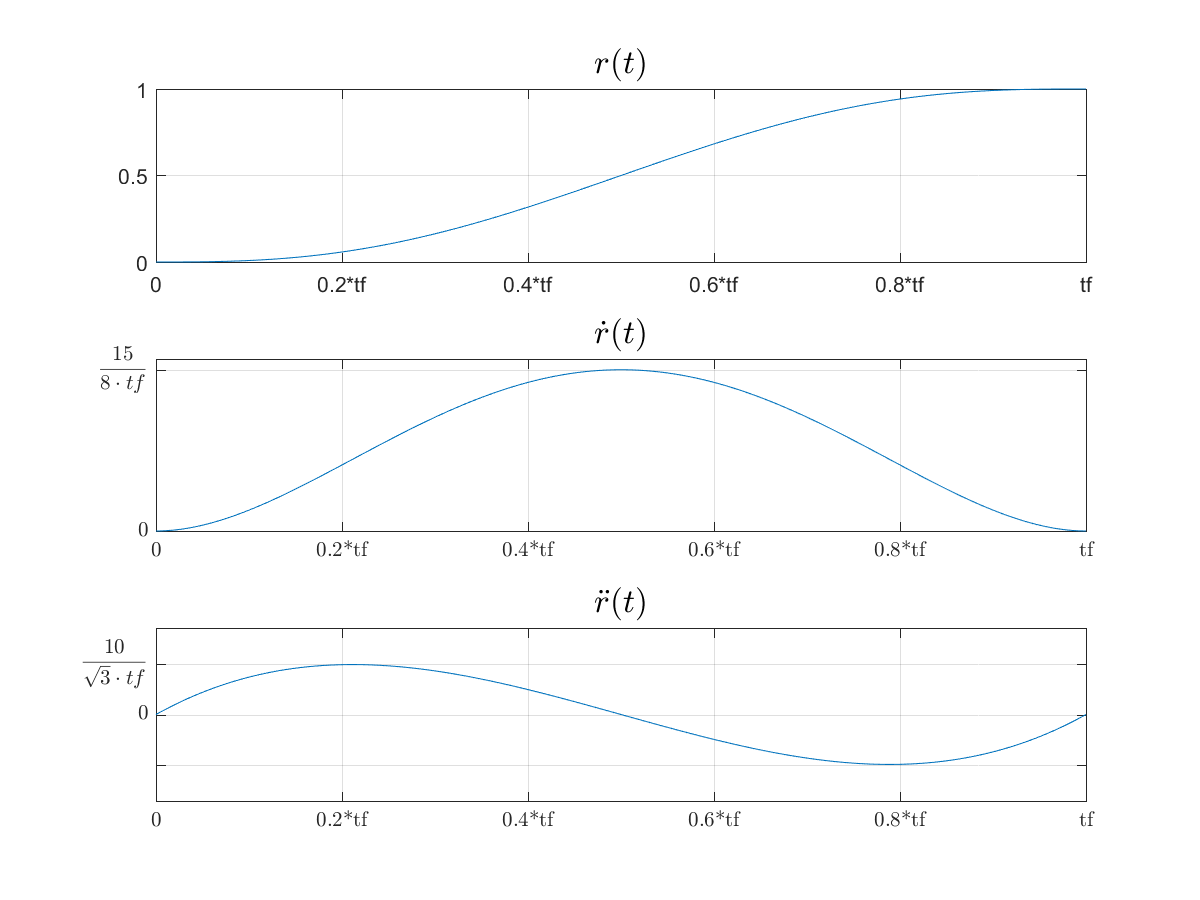
\includegraphics[width=\textwidth]{TrajFig2.png}
	\caption{r(t) et ses d\'{e}riv\'{e}s}
	\label{eller2}
\end{figure}

La trajectoire dans l'espace est montr\'{e}e dans la figure \ref{eller3}. Les points sont espac\'{e}s d'un m\^{e}me intervalle de temps afin d'indiquer l'effet de la vitesse sur la trajectoire.

\begin{figure}[H]
	\centering	%Botar a figura aqui
	\captionsetup{justification=centering,margin=1cm}
	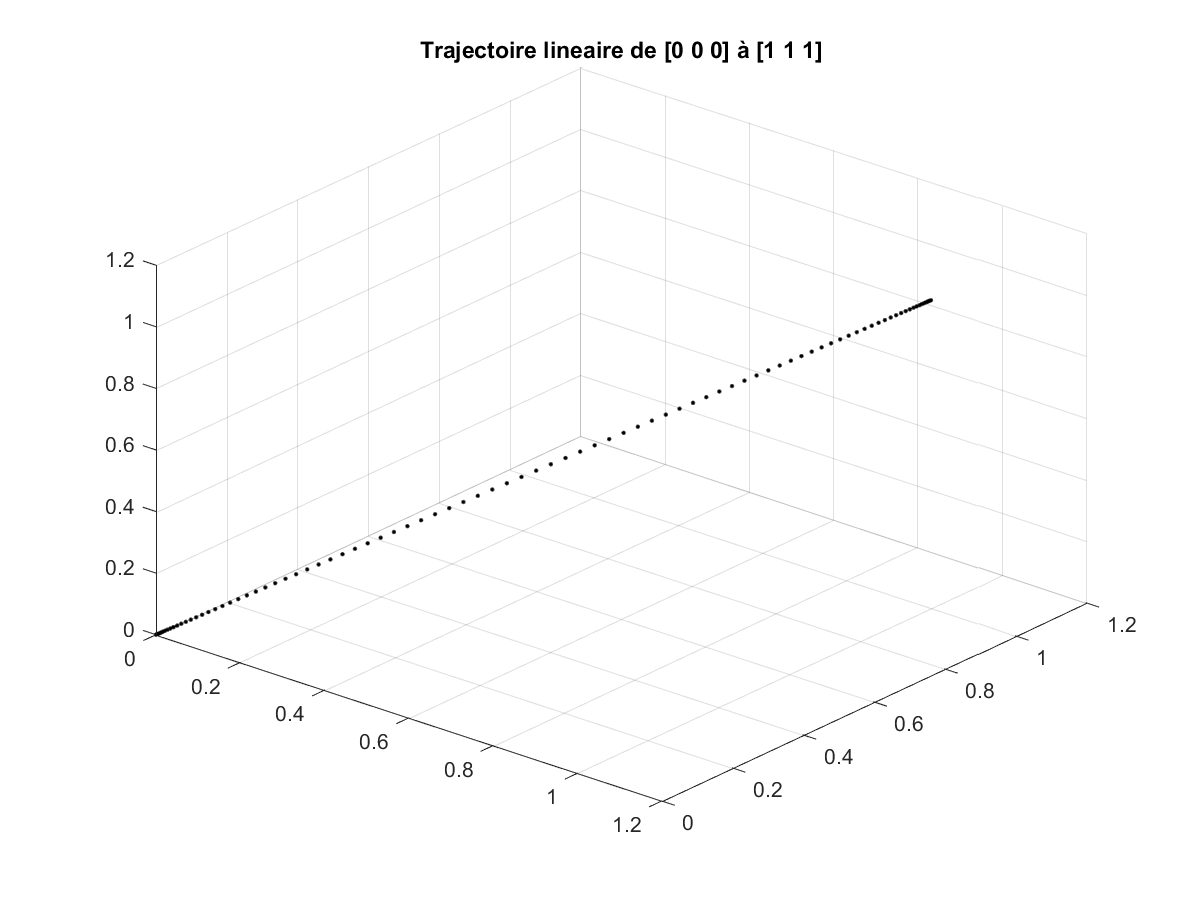
\includegraphics[width=8cm]{TrajFig3.png}
	\caption{Trajectoire lineaire dans l'espace}
	\label{eller3}
\end{figure}

\mysubsubsection{Trajectoire Circulaire}

Une des trajectoires souhait\'{e}es c'est la trajectoire circulaire dans l'espace. Avec les m\^{e}mes principes de conception de la trajectoire lin\'{e}aire on va d\'{e}finir une courbe dans l'espace et la suivre avec un profil de position donn\'{e} par un polyn\^{o}me de ${5}^{\grave{e}me}$ d\'{e}gr\'{e}e, afin de suivre une circonf\'{e}rence dans l'espace de temps entre 0 e $t_f$. On utilisera la fonction $r(t)\ ,\ $d\'{e}finie auparavant.

La courbe sera d\'{e}finie par l'utilisateur parmi trois points, que, sauf en cas de colin\'{e}arit\'{e}, d\'{e}finissent toujours un cercle dans l'espace. Une fois d\'{e}fini en termes d'un rayon R et d'un centre${\boldsymbol{\ }\boldsymbol{p}}^{\boldsymbol{c}}$ on peut d\'{e}finir la trajectoire dans le temps, dont expression est donn\'{e} ci-dessous~: 

\[\boldsymbol{p}\left(t\right)={\boldsymbol{p}}^{\boldsymbol{c}}+\left[ \begin{array}{c}
\begin{array}{c}
R{\mathrm{cos} (2\pi \ r\left(t\right)+{\varphi }_0)\ } \\ 
R\ {\mathrm{sin} (2\pi \ r\left(t\right)+{\varphi }_0)\ } \end{array}
\end{array}
\right]\] 

\vspace{3pt}
Dont le condition limite est~:$\boldsymbol{\ }\boldsymbol{\ }{\boldsymbol{p}}^{\boldsymbol{c}}+\left[ \begin{array}{c}
\begin{array}{c}
R{\mathrm{cos} ({\varphi }_0)\ } \\ 
R\ {\mathrm{sin} ({\varphi }_0)\ } \end{array}
\end{array}
\right]=\ {\boldsymbol{p}}^{\boldsymbol{i}}$\textbf{ }(Point initial)

\bigbreak

L'expression est donn\'{e}e en termes du plan x y, mais le r\'{e}sultat est g\'{e}n\'{e}ral, une fois qu'il faut seulement multiplier les points r\'{e}sultants par des matrices de rotation pour obtenir une configuration n'importe quelle, ce qui est en effet la m\'{e}thode utilis\'{e}e lors de la mise en {\oe}uvre.

La vitesse dans la direction du mouvement est donn\'{e}e par~:
\[\left\|\frac{d\bm{p}(t)}{dt}\right\|=\ \ \sqrt{{\left(\frac{dp_x(t)}{dt}\right)}^2+{\left(\frac{dp_y(t)}{dt}\right)}^2}=2\pi R\ r(t)\] 
Ce qui veut dire que la vitesse, bien comme l'acc\'{e}l\'{e}ration, sont limit\'{e}es e peuvent \^{e}tre facilement r\'{e}gl\'{e}es en termes de vitesses ou acc\'{e}l\'{e}rations maximales. La figure \ref{eller4} montre la trajectoire dans l'espace, o\`{u} les points sont espac\'{e}s d'un m\^{e}me intervalle de temps afin de montrer la variation de la vitesse au long de la courbe. 

\begin{figure}[H]
	\centering
	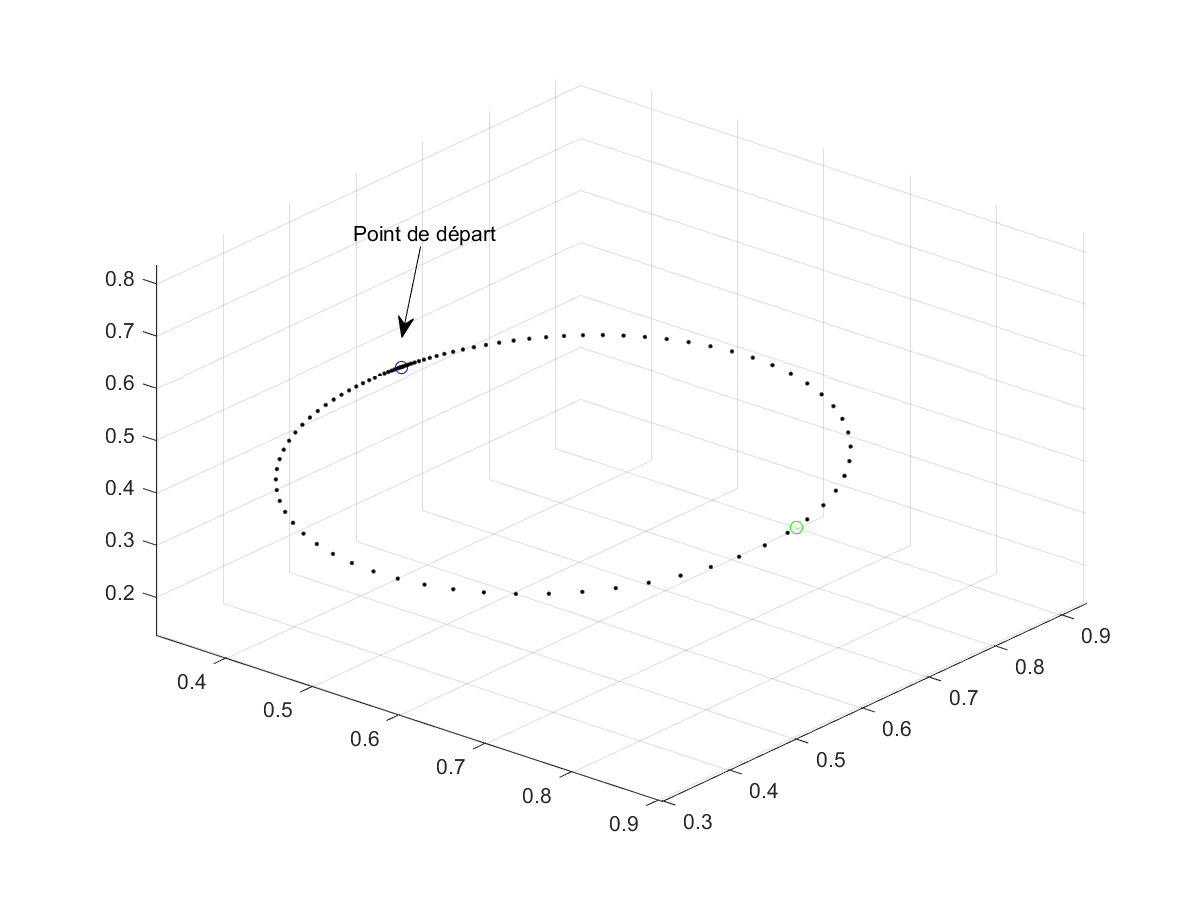
\includegraphics[width=8cm]{TrajFig4.png}
	\caption{Trajectoire circulaire dans l'espace}
	\label{eller4}	
\end{figure}

Et la figure \ref{eller5} montre les positions, vitesses et acc\'{e}l\'{e}rations par rapport au centre du cercle.  

\begin{figure}[H]
	\captionsetup{justification=centering,margin=1cm}
	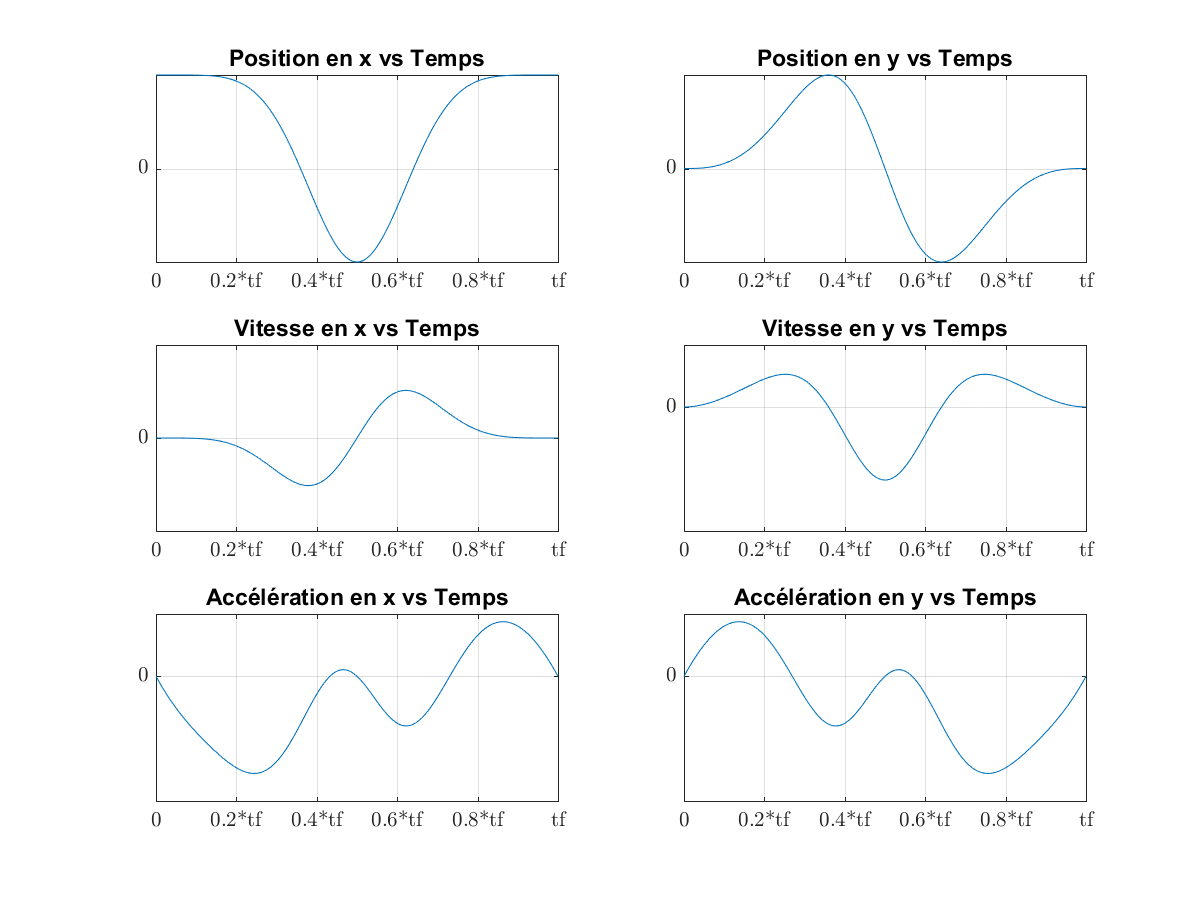
\includegraphics[width=\textwidth]{TrajFig5.png}
	\caption{Positions, vitesses et acc\'{e}l\'{e}rations en x et y}
	\label{eller5}
\end{figure}


En plus, si l'utilisateur donne un point initial${\boldsymbol{\ }\boldsymbol{p}}^{\boldsymbol{i}}$, un point final ${\boldsymbol{p}}^{\boldsymbol{f}}$ et un point interm\'{e}diaire ${\bm{p}}^{\bm{m}}$ on peut d\'{e}finir la trajectoire d'arc de cercle qui passe pour ces trois points.  
\[\bm{p}\left(t\right)={\bm{p}}^{\bm{c}}+\left[ \begin{array}{c}
\begin{array}{c}
R{\mathrm{cos} (\left[{\varphi }_f{-\varphi }_0\right].r\left(t\right)+{\varphi }_0)\ } \\ 
R\ {\mathrm{sin} (\left[{\varphi }_f{-\varphi }_0\right].r\left(t\right)+{\varphi }_0)\ } \end{array}
\end{array}
\right]\] 
O\`{u} la nouvelle condition limite est : 
 \[{\boldsymbol{p}}^{\boldsymbol{c}}+\left[ \begin{array}{c}
\begin{array}{c}
R{\mathrm{cos} ({\varphi }_f)\ } \\ 
R\ {\mathrm{sin} ({\varphi }_f)\ } \end{array}
\end{array}
\right]=\bm{p}\left(t_f\right) = {\bm{p}}^{\bm{f}}\]

O\`{u} une fois de plus, on a repr\'{e}sent\'{e} la courbe dans le plan x y. La figure \ref{eller6} montre un exemple de ce genre de trajectoire de fa\c{c}on g\'{e}n\'{e}rale.


\begin{figure}[H]
	\centering
	\captionsetup{justification=centering,margin=1cm}
	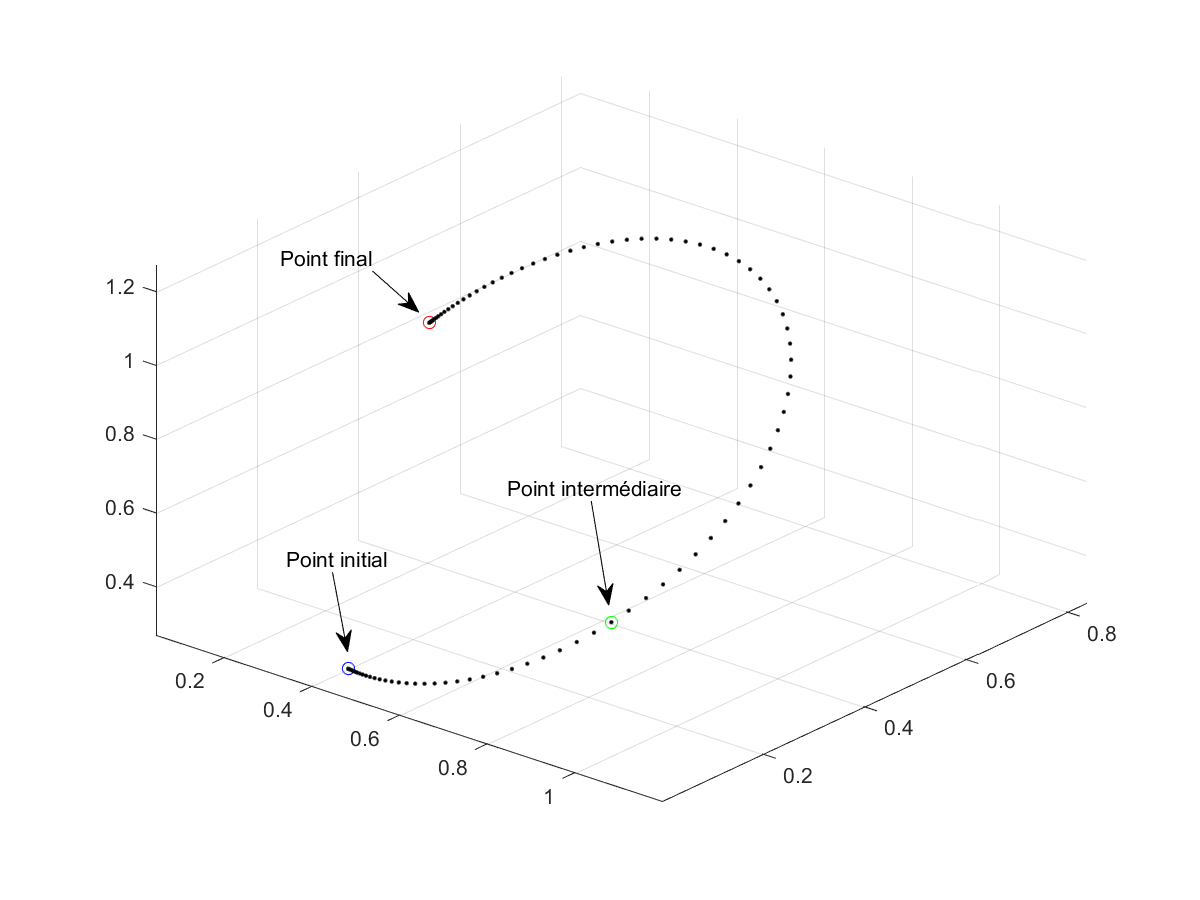
\includegraphics[width=8cm]{TrajFig6.png}
	\caption{Trajectoire d'arc de cercle dans l'espace}
	\label{eller6}
\end{figure}
